\chapter{Plataforma de desarrollo}
\label{cap:capitulo4}


\begin{flushright}
\begin{minipage}[]{10cm}
\emph{Cuando quieres algo, todo el universo conspira para que realices tu deseo}\\
\end{minipage}\\

Paulo Coelho, \textit{El Alquimista}\\
\end{flushright}

\vspace{1cm}

En este capítulo, se explicará con detalle todas las herramientas tanto a nivel hardware como software que han sido utilizadas para poder desarrollar el proyecto.


\section{Hardware}
\label{sec:hardware}

En esta sección se descibirán todos los componentes físicos que han sido utilizados en este trabajo, los cuales han sido adquiridos en su mayor parte por el precio y la funcionalidad que tienen.\\ \\
A continuación se explicará con detalle aquellos que están presentes en esta arquitectura hardware.

\subsection{Micrófono micro USB}
\label{subsec:micro}

Se trata de un tipo de micrófono(Figura \ref{fig:microfono-usb}), el cual es utilizado para la grabación de audio compatible con puertos USB y teniendo un pequeño tamaño y peso lo cual lo hace ideal para incorporarlo en la Raspberry. 


Se llegó a la conclusión de que era la mejor idea usar este tipo de micrófono, ya que no necesita clabes por lo que facilita al usuario comunicarse con el dispositivo siendo más cómodo para él. Además de ser bajo coste, tiene un precio que ronda los 10 \euro, es fácil de adquirir en páginas web como Amazon. Este tipo de micrófono tiene 2 metros de distancia efectiva y filtra el ruido de fondo no deseado, haciendo que el sonido sea más claro y limpio.


\begin{figure}[H] % Usa [H] para forzar la posición
  \begin{center}
    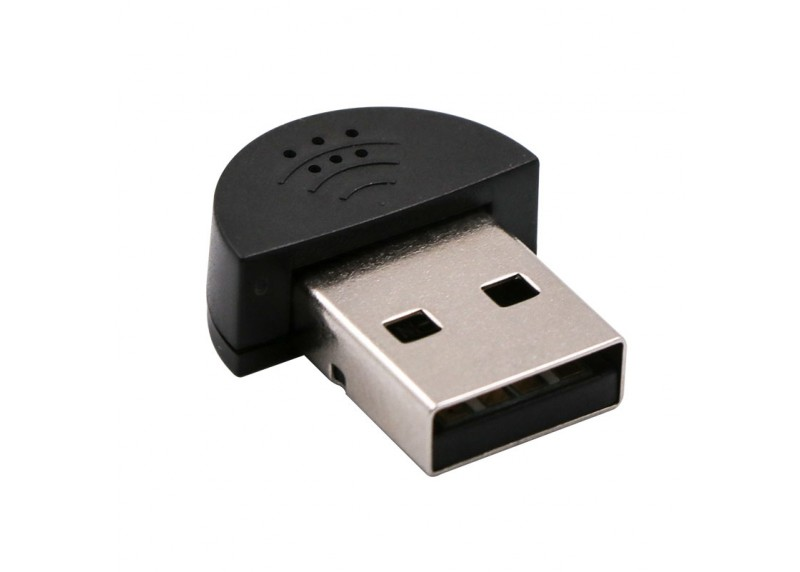
\includegraphics[scale=0.3]{figs/microfono-usb}
  \end{center}
  \caption{Micrófono micro USB.}
  \label{fig:microfono-usb}
\end{figure}


\subsection{Controlador driver L298N}
\label{subsec:l298n}

Un controlador de motor o driver(Figura \ref{fig:l298n}) sirve para controlar motores de corriente continua(DC) o motores paso a paso el cual, permite sobre todo controlar tanto la velocidad como la dirección de estos motores. Este módulo hardware tiene la capacidad de transformar las señales lógicas las cuales les envía el procesador a una serie de pulsos de potencia que alimentarán ambas bobinas de cada motor reductor para hacer girar cada uno de ellos en un orden concreto. A parte, dispone de protecciones para que no se dañe en el caso de que se haga un mal uso del mismo, y siendo su precio original por solo 3 \euro.\\ 

El control del mismo es simple, primero habría que conectar el positivo de la fuente de alimentación externa de 6 V a los 12 V de la placa(Vin), y teniendo el jumper de selección de 5 V activo, ya que el módulo permite una alimentación de entre 6 - 12V y si el jumper se encuentra inactivo, se permite una alimentación de 12 - 35V pero no sería necesario en este caso ya que el motor sólo necesita 6V. \\

Se recomienda no conectar nunca una tensión de entrada al pin de más de 5V cuando el jumper de 5V se encuentre activado, ya que provocaría un cortocircuito y podría dañar permanentemente el módulo. Luego, el negativo de la fuente externa tiene que ir al GND de la placa y desde este mismo, saldrá otro cable que irá al GND de la Raspberry.\\ \\ \\

Finalmente, los pines de salida de la placa deben ir conectados a los pines de las bobinas de cada motor y los pines de entrada IN1 - IN4 irán conectados a los diferentes pines \hyperlink{GPIO}{GPIO} de la Raspberry. Si no se desactivan los jumpers de activación (ENA y ENB), ambos motores girarán a su máxima velocidad, por lo que habrá que desactivarlos para poder configurar la velocidad a la que se quiere que vaya cada motor.

\begin{figure}[H]
  \centering
  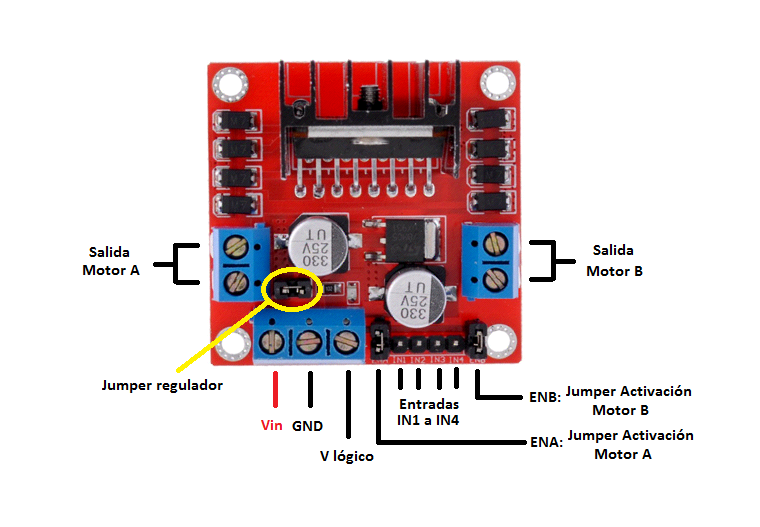
\includegraphics[scale=0.6]{figs/L298N} % Escala la imagen al 150% de su tamaño original
  \caption{Controlador driver L298N.}
  \label{fig:l298n}
\end{figure}

\begin{table}[H]
\begin{center}
\begin{tabular}{|c|c|}
\hline
\textbf{Parámetros} & \textbf{Valores} \\
\hline
Nombre del controlador & L298N \\
Voltaje de alimentación & 6 - 12 V(jumper) \\
Interfaz de comunicación & Pines digitales, CFG y \hyperlink{PWM}{PWM} \\
Corriente máxima de fase(RMS) & 2 x 2 A \\
Pérdida de conducción & 0.9 - 1.5~$\Omega$ \\
Voltaje lógico & 5 V \\
Dimensiones & 5 x 5 x 3 cm \\
Peso & 27 g \\
\hline
\end{tabular}
\caption{Especificaciones técnicas del L298N}
\label{cuadro:ejemplo}
\end{center}
\end{table}

\vspace{2cm}

\subsection{Motores}
\label{subsec:motores}

Un motor reductor es un tipo de motor eléctrico que tiene incorporado un mecanismo de reducción como un engranaje y que sirve para aumentar el torque de salida, es decir, una mayor fuerza en el eje del motor, lo cual es una opción idónea para esta aplicación ya que se necesita mover mucho peso contando con las piezas del robot, la Powerbank, la Raspberry y la batería, disminuyendo la velocidad de rotación y teniendo a su vez un control preciso del motor. La velocidad en este caso no menos importante que la fuerza del motor ya que el objetivo final que pueda desplazarse con todo el peso incorporado para llegar al objetivo final aunque será necesaria controlarla igualmente. \\

En concreto, se han usado dos motores reductores como los que se muestran en la Figura \ref{fig:Motor} junto con dos ruedas de anclaje que encajan perfectamente con los ejes de cada motor, y están a la venta en Amazon por un precio de 11 \euro. 

\begin{figure}[H]
  \centering
  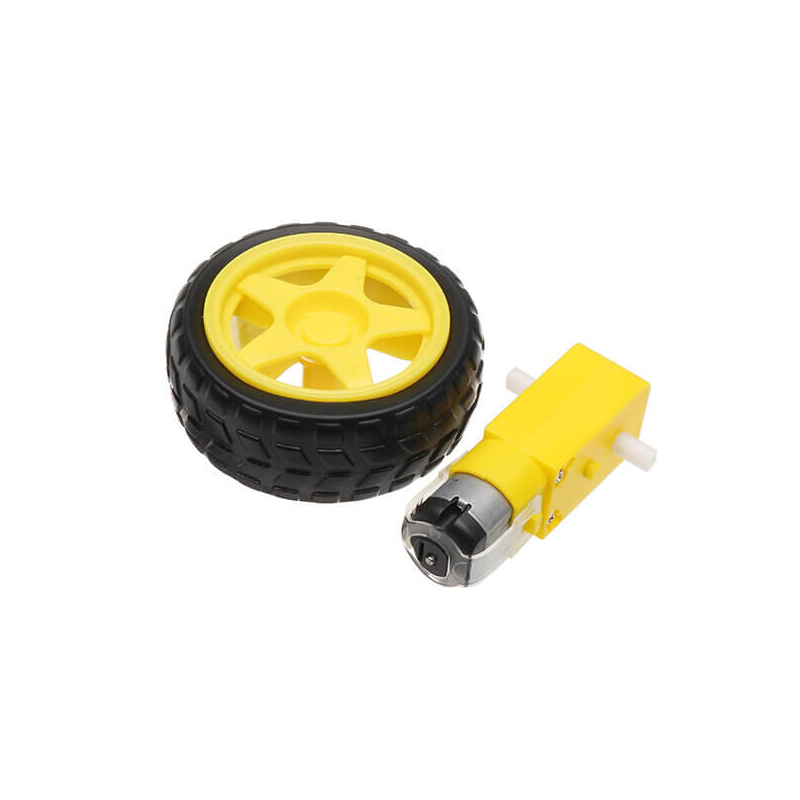
\includegraphics[scale=0.35]{figs/motor} % Escala la imagen al 150% de su tamaño original
  \caption{Motor reductor con rueda de anclaje.}
  \label{fig:Motor}
\end{figure}

\begin{table}[H]
\begin{center}
\begin{tabular}{|c|c|}
\hline
\textbf{Parámetros} & \textbf{Valores} \\
\hline

Nombre del motor & Motor reductor \\
Peso & 20 g \\  
Diámetro del eje & 3 mm \\   
Dimensiones & 70 x 22 x 18mm \\   
Torque de sujeción & 0.0687 Nm Aprox \\
Corriente máxima de fase & 850 mA \\  
Tipo de motor & Corriente continua \\   
Voltaje & 3 - 6 V \\  
Reducción & 48:1 \\ 
Velocidad sin carga & 230 rpm \\ 


\hline
\end{tabular}
\caption{Especificaciones técnicas de los motores}
\label{cuadro:ejemplo}
\end{center}
\end{table}


\subsection{Fuentes de alimentación}
\label{subsec:fuentes_alimentacion}

Para poder alimentar al controlador L298N, se va a necesitar una batería de 6 V y 6 A y que sea recargable como la que se muestra en la 
en la figura \ref{fig:bateria}, ya que se será necesaria su recarga para hacer múltiples pruebas con el robot. Esta batería consta de 5 pilas AA y un cable de carga, con un peso de 129 gramos, lo cual es perfecta para que pueda proporcionar la potencia necesaria para los motores y que a diferencia de las baterías de ácido son más ligeras, ya que éstas, normalmente son más pesadas debido a que están hecas de plomo y ácido.\\

Este tipo de fuentes, se pueden encontrar en páginas como Amazon a un precio de 18 \euro, pero se podían haber usado otras que proporcionasen una alimentación en el rango de 6 - 12 V, siempre y cuando se tenga el jumper del controlador inactivo, porque si estuviese activoo habría que proporcionar una alimentación entre 12 - 35 V como se mencionó anteriormente, pero como los motores necesitan 6 V sólo, pues valdrían con las que se han usado. \\

Por otra parte, habría que alimentar a la Raspberry, ya que el robot se manejará de manera independiente y sin cables de por medio, por lo que se utilizará una Powerbank como la de la figura \ref{fig:Powerbank}, la cual es idónea debido a su peso ligero de 200 gramos y la tensión y amperaje que proporciona de 5 V y 3 A respectivamente, ya que es justo lo que necesita la Raspberry Pi 4 que se va a utilizar para que funcione correctamente y tenga un rendimiento estable.

\begin{figure}[H]
  \begin{minipage}{0.48\textwidth}
    \centering
    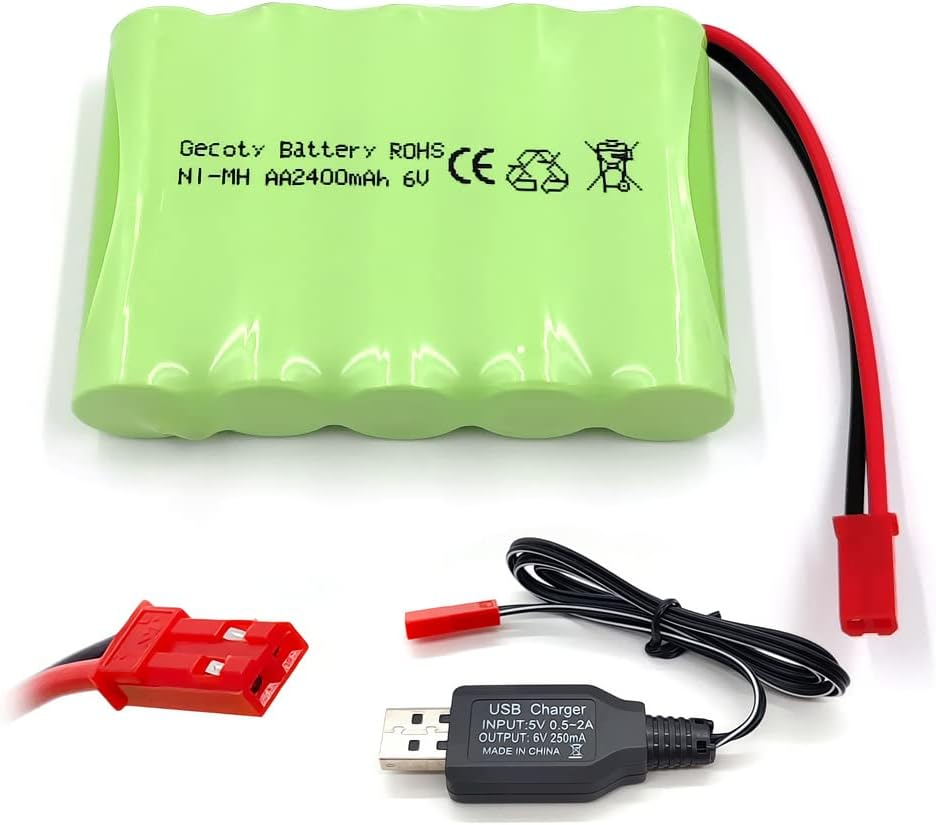
\includegraphics[width=6.5cm]{figs/bateria.jpg}
    \caption{Batería recargable con cable de carga.}
    \label{fig:bateria}
  \end{minipage}
  \hfill
  \begin{minipage}{0.48\textwidth}
    \centering
    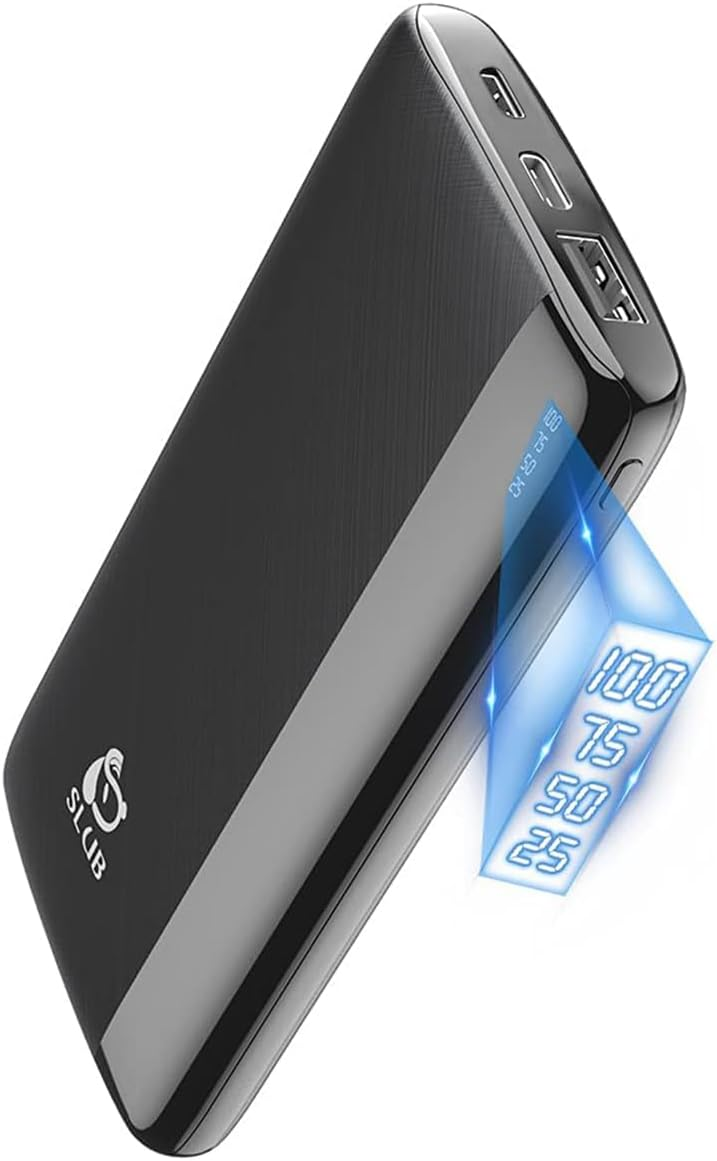
\includegraphics[scale=0.13]{figs/powerbank.jpg}
    \caption{Powerbank.} 
    \label{fig:Powerbank}
  \end{minipage}
\end{figure}

\subsection{Rueda loca}
\label{subsec:rueda_loca}

Para que el robot pueda desplazarse en cualquier dirección sin ningún problema se utilizará una rueda loca como la de la figura \ref{fig:Rueda_loca} imitando el comportamiento de una pelota rodante, la cual irá anclada en la parte trasera del robot con 2 tornillos y 2 tuercas proporcionando al robot un movimiento suave y de baja fricción, de alto rendmiento y larga vida.


\begin{figure}[H]
  \centering
  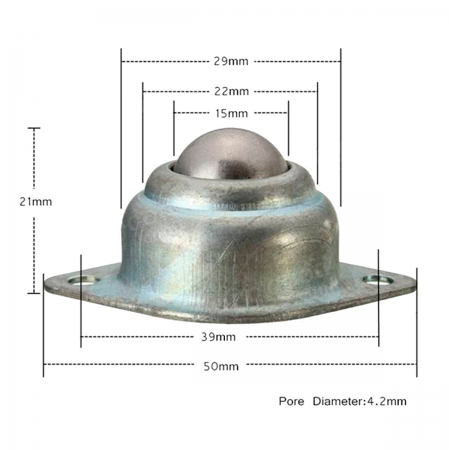
\includegraphics[scale=0.4]{figs/rueda_loca} % Escala la imagen al 150% de su tamaño original
  \caption{Rueda loca para robot.}
  \label{fig:Rueda_loca}
\end{figure}



\subsection{Base principal}
\label{subsec:base_principal}

Primero, habría que pensar en la forma que tiene que tener la base para poder soportar tanto los motores, como la batería, la Raspberry y la Powerbank. Para ello, se diseñará una estructura muy simple en la cual, habrá diferentes cavidades las cuales nos servirán para poder insertar de la manera más fácil posible todo lo que se necesita, como lo mencionado anteriormente más el controlador, sensores, cables y otros huecos para añadir si se requiere en un futuro otro tipo de sensores y actuadores. \\

Finalmente, para el diseño de esta base, habría que hacer uso de FreeCAD \ref{subsec:freecad} para poder imprimir esta pieza y cumplir con el objetivo establecido inicialmente de poder soportar todo el peso posible, y que sea escalable a nivel de que se puedan cualquier cosa para cumplir con objetivos futuros y de esta manera también, al ser completamente Open Source, cualquier persona podrá modificarlo a su manera y utilizarlo de manera gratuita, por lo que quedaría de la siguiente manera como se puede apreciar en esta figura \ref{fig:Base_principal}:

\begin{figure}[H]
  \centering
  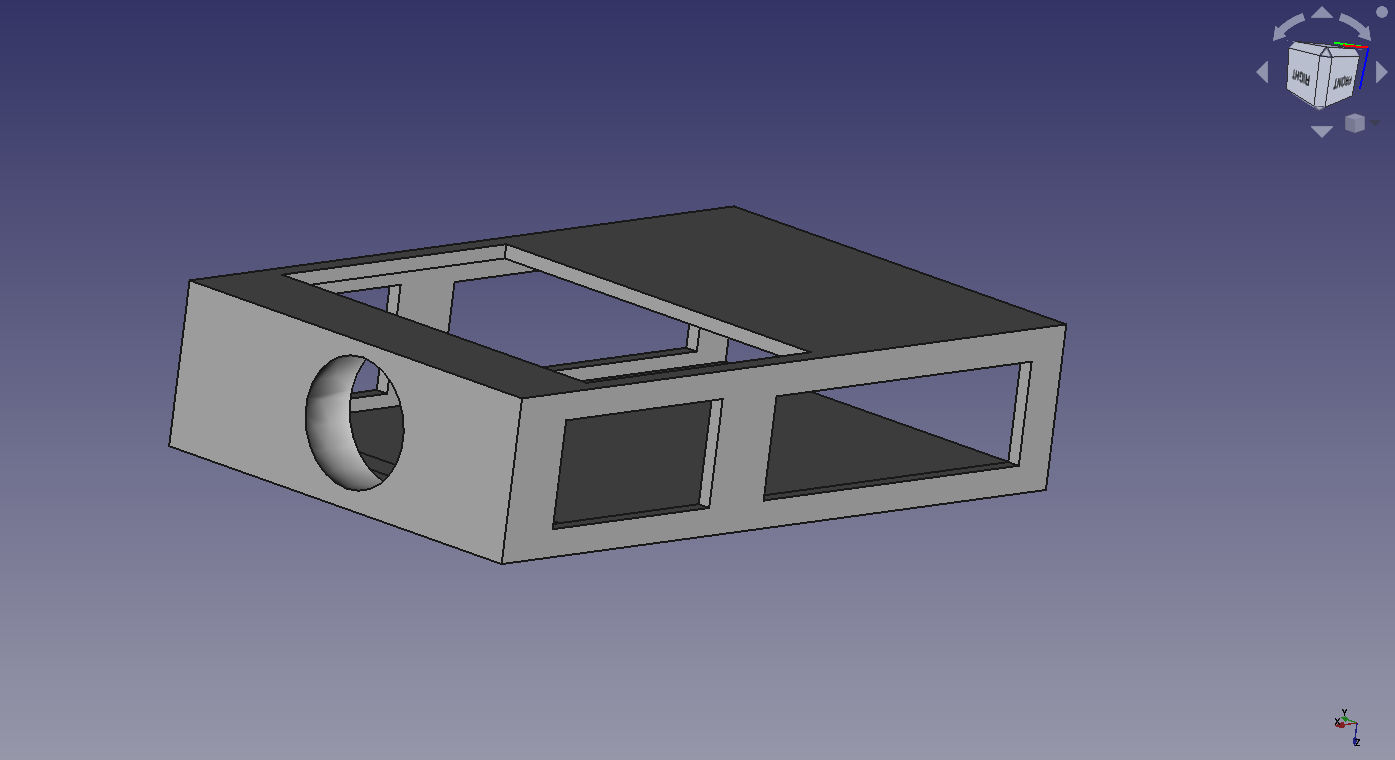
\includegraphics[scale=0.25]{figs/base} % Escala la imagen al 150% de su tamaño original
  \caption{Base principal.}
  \label{fig:Base_principal}
\end{figure}

Como se puede apreciar en la imagen, la cavidad circular sirve por si en algún futuro se desea añadir algún sensor, ya sea como el ultrasonidos. Las dos cavidades rectangulares menores sirven para poder anclar las ruedas a los motores que irán éstos a su vez añadidos a través del hueco rectangular superior. Por otra parte, las dos cavidades rectangulares mayores, junto con el hueco de la parte trasera, sirven para poder introducir la batería y el magnetómetro como se verá más adelante de una manera asequible y sencilla. La Raspberry y la Powerbank irán encima de la parte trasera y el controlador y los cables como no hace faltan que estén sujetos a nada debido a menor peso, irán en el hueco frontal superior encima de los motores.


\subsection{Plataforma hardware}
\label{subsec:plataforma_hardware}


Para poder cumplir con el objetivo establecido de diseñar y controlar un robot guía por voz, con las características que ya se han definido en el capítulo anterior y que a sea también de bajo coste, en este proyecto la infraestrucutra hardware se ha centrado en los sistemas embebidos que hay disponibles en el mercado. En primer lugar, una parte del software, como la de entrenar la red neuronal, se probó con éxito en un sistema operativo Ubuntu 20.04 y el siguiente paso era migrarlo a la Raspberry Pi. En segundo lugar, se intentó probar que funcinonara en una Raspberry Pi 3 Model B+ pero sin éxito, ya que aunque se consiguieron instalar los mismos paquetes con las mismas versiones sin ningún problema, a la hora de instalar en concreto una de las librerías necesarias para transformar y manipular los archivos de audio como la de librosa, se experimentaron problemas de bloqueos y de rendimiento durante días sin ningún cambio apreciable, por lo que seguramente sea por limitaciones de recursos de hardware de este modelo.\\

La Raspberry Pi 3+ tiene especificaciones decentes para muchas tareas, pero ciertas aplicaciones y bibliotecas pueden ser exigentes en términos de procesamiento y memoria, lo que puede conllevar a problemas de rendimiento. La biblioteca librosa es conocida por ser computacionalmente intensiva, especialmente al trabajar con archivos de audio grandes o al realizar operaciones complejas de procesamiento de señales de audio, por lo que se esta opción queda descartada y se llegará a probar en una Raspberry Pi 4 Model B.\\

En general, la Raspberry Pi 4 ofrece un salto significativo en términos de rendimiento y capacidades en comparación con la Raspberry Pi 3 Model B+, ya que tiene un procesador más potente y mucha más RAM (4 GB), lo que la hace más capaz de manejar tareas intensivas y ejecutar aplicaciones más exigentes. Para usarla correctamente, habrá que añadir disipadores de calor y un ventilador, ya que genera más calor que la Raspberry Pi 3.



\begin{figure}[H]
  \centering
  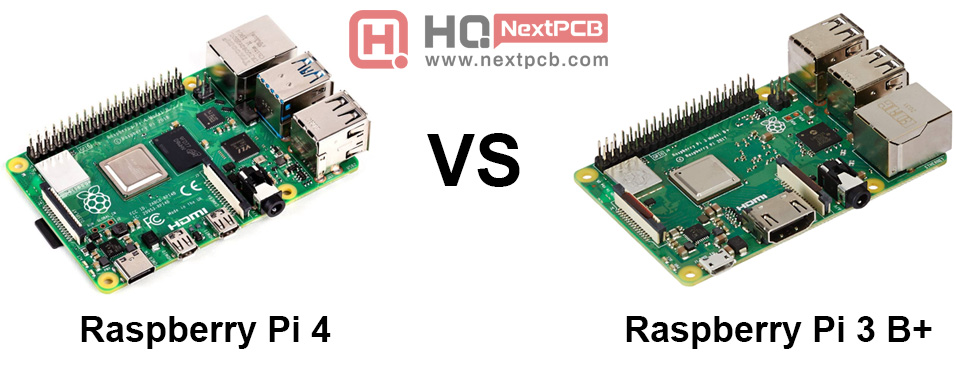
\includegraphics[scale=0.4]{figs/rasps} % Escala la imagen al 150% de su tamaño original
  \caption{Raspberry Pi 4B vs Raspberry Pi 3B+.}
  \label{fig:Raspberry}
\end{figure}


Esta placa tiene pines \hyperlink{GPIO}{GPIO} los cuales permiten que se conecten tanto sensores como actuadores mediante diferentes tipos, como los que se muestran en la figura \ref{fig:Pines}. Hay diferentes tipos de pines:

\begin{itemize}
 \item \textit{GND.} Es usado para poder cerrar el circuito elécctrico y que la corriente pueda fluir adecuadamente entre los dispositivos conectados y no haya ningún daño. Son los pines 6,9,14,20,25,30,34 y 39.
 \item \textit{Pin de 5V.} En los pines 2 y 4 se proporciona una alimentación de 5V.
 \item \textit{Pin de 3V.} En los pines 1 y 17 se proporciona una alimentación de 3V.
 \item \textit{Modulación por ancho de pulso (\hyperlink{PWM}{PWM}).} Se corresponden con los pines 12,32,33 y 35 y permiten modificar el ciclo de tranajo con una señal periódica establecida.
 \item \textit{Conexión \hyperlink{UART}{UART}.} Se corresponden con los pines 8 y 10.
 \item \textit{Conexión \hyperlink{SPI}{SPI}.} Se corresponden con los pines 19,21,23,24 Y 26.
 \item \textit{Conexión \hyperlink{I2C}{I2C}.} Se corresponden con los pines 3(SDA), 5(SCL), 27(SDA) y 28(SCL).	
 \item \textit{} Los demás pines son usados para garantizar la conexión de entrada o salida con el dispositivo conectado. 
\end{itemize}\

\begin{figure}[H]
  \centering
  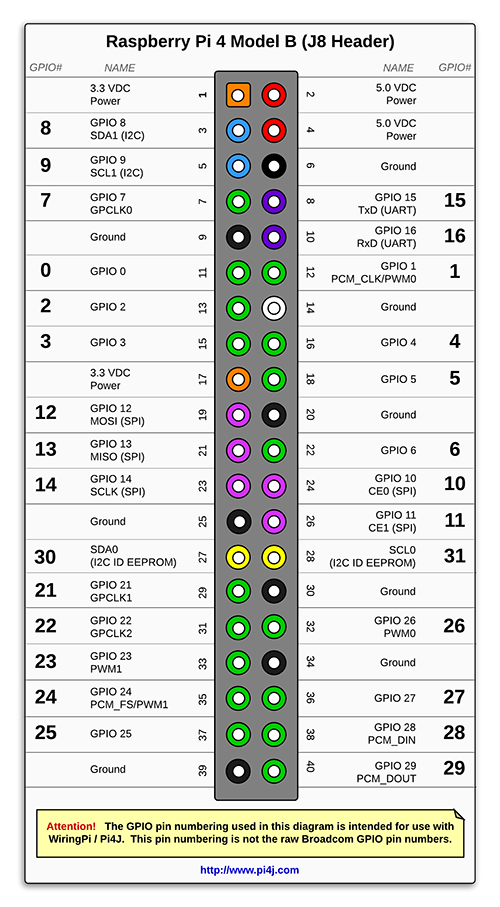
\includegraphics[scale=0.4]{figs/pines} % Escala la imagen al 150% de su tamaño original
  \caption{Diferentes tipos de pines GPIO en Raspberry Pi 4B.}
  \label{fig:Pines}
\end{figure}


\subsection{Magnetómetro}
\label{subsec:magnetómetro}


Para obtener la orientación absoluta del robot se puede usar un sensor como ya se mencionó anteriormente como el mpu9250 que se aprecia en la figura \ref{fig:mpu9250}. Este dispositivo compacto y versátil que combina el acelerómetro de 3 ejes, el giroscopio de 3 ejes y el magnetómetro de 3 ejes en un solo paquete,es decir, por lo puede medir la aceleración lineal, la velocidad angular y la intensidad del campo magnético terrestre en los 3 ejes.\\ \\ Tiene integrado un \hyperlink{DMP}{DMP} capaz de realizar complejos algoritmos de captura de movimiento de los 9 ejes. Este sensor se comunica con microcontroladores a través de la interfaz I2C y posee una librería muy extensa para su uso inmediato e incorpora un regulador de voltaje a 3.3V en la placa y resistencias pull-up para su uso directo por I2C. Para una captura precisa de movimiento rápido y lento, tiene un rango de escala programable de 250/500/1000/2000 grados/seg para el giroscopio, 2g/4g/8g/16g para el acelerómetro y ±4800µT para el magnetómetro.\\ \\
Su magnetómetro incorporado se puede utilizar para estimar el ángulo de orientación absoluta como el de una brújula. Este ángulo conocido como acimut, se refiere a la dirección en la que apunta un objeto o una persona, en relación normalmente con el norte.\\ \\ Una lectura de 0º indicaría una dirección hacia el norte verdadero, 90º, 180º y 270º indicarían este, sur y oeste, respectivamente. Se puede determinar este ángulo utilizando lecturas de un magnetómetro con otras técnicas de calibración para estimar con alta precisión en qué dirección va, resultando así muy útil para que el robot pueda orientarse en interiores.



\begin{figure}[H]
  \centering
  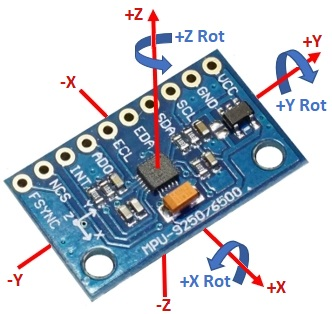
\includegraphics[scale=0.7]{figs/mpu9250} % Escala la imagen al 150% de su tamaño original
  \caption{Sensor MPU9250.}
  \label{fig:mpu9250}
\end{figure}


\begin{table}[H]
\begin{center}
\begin{tabular}{|c|c|}
\hline
\textbf{Parámetros} & \textbf{Valores} \\
\hline

Nombre del sensor & MPU9250 \\
Voltaje de operación & 3.3 - 5 V \\  
Grados de libertad(\hyperlink{DoF}{DoF}) & 9 \\   
Rango de acelerómetro & ±2g, ±4g, ±8g, ±16g \\   
Rango Giroscopio & ±250º/Seg, ±500º/Seg, ±1000º/Seg, ±2000º/Seg \\
Rango Magnetómetro & ±4800 $ \mu $T \\  
Interfaz & I2C y SPI \\   
Conversor AD & 16 Bits (salida digital) \\   
Dimensiones & 25 x 16 x 3mm \\
Consumo de energía(modo activo) & 3.2 mA \\
Temperatura de funcionamiento & -40ºC a +85ºC \\ 


\hline
\end{tabular}
\caption{Especificaciones técnicas del sensor MPU9250}
\label{cuadro:ejemplo}
\end{center}
\end{table}

\section{Software}
\label{sec:software}


Al hacer uso finalmente de una Raspberry Pi 4B, se usó un sistema operativo oficial Raspberry Pi OS conocido como Raspbian(Figura \ref{fig:raspbian}) con la versión de 64 bits y como está basado en Debian, se dispondrá de las cualidades de un sistema Linux. Se ha decidido usar este sistema operativo debido a su optimización para que pueda funcionar en procesadores ARM(el que ya tiene la Raspberry) ofreciendo así el mejor rendimiento posible para este placa.


Posteriormente, se definirán todos las librerías externas y programas que han sido necesarios para poder desarrollar este proyecto correctamente.

\begin{figure}[H]
  \centering
  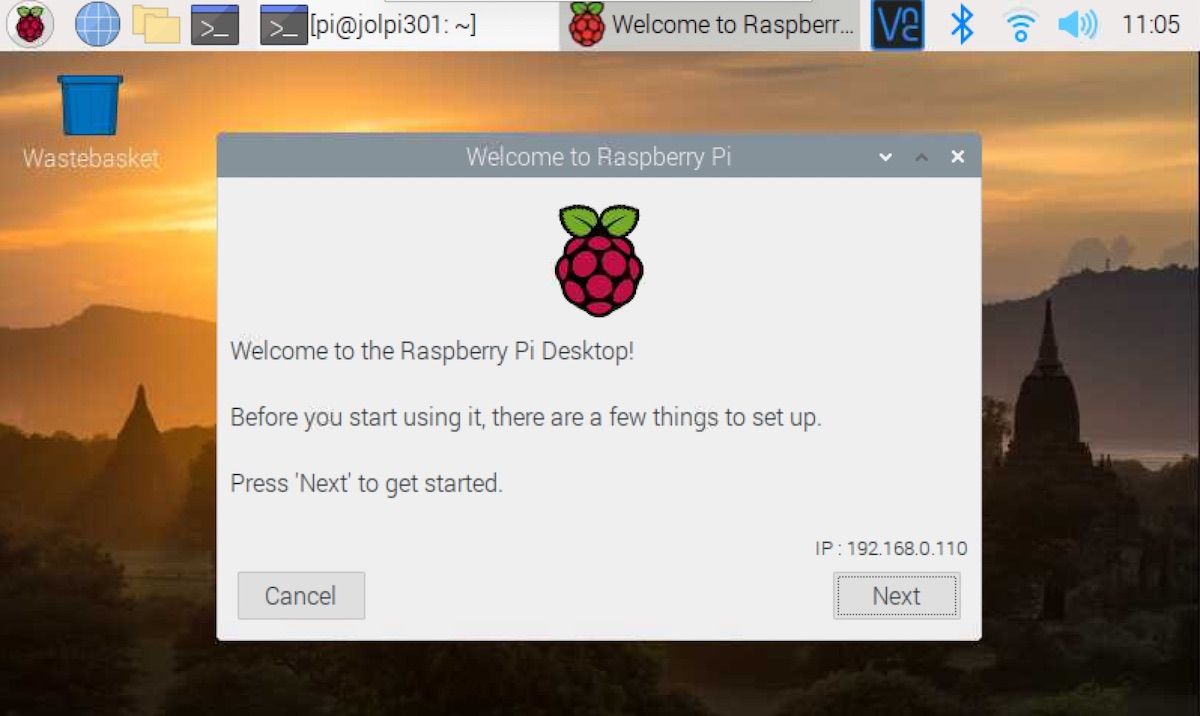
\includegraphics[scale=0.3]{figs/raspbian} % Escala la imagen al 150% de su tamaño original
  \caption{Raspberry Pi OS.}
  \label{fig:raspbian}
\end{figure}


\subsection{Python}
\label{subsec:python}

Python es un lenguaje de programación interpretado de alto nivel y orientado a objetos, es decir, que al ser de alto nivel su nivel de abstracción es más cercano al lenguaje humano que al de una máquina y es de fácil uso en comparación con los lenguajes de bajo nivel. Es interpretado en el sentido que es un intérprete el que ejecuta línea por línea en vez de ser compilado a código máquina previamente como en C o C++. Es uno de los lenguajes de programación más usados en el mundo debido a su amplia librería estándar, garantizando así multitud de funciones y módulos para realizar difentes tareas y a suz vez, está soportado de manera nativa por el sistema operativo utilizado Raspbian.\\ \\ También cuenta con una gran variedad de librerías de terceros como Numpy para cálculos numéricos, Pandas para el análisis de datos, librosa para la manipulación de datos de auido lo cual será de gran ayuda a la hora de entrenar la red neuronal con los comandos, seaborn para la visualización de datos estadísticos, entre otros. En este proyecto, Python se usará para leer y procesar los datos de los sensores de manera concurrente proporcionando órdenes a los actuadores para alcanzar un objetivo en concreto.



\subsection{FreeCAD}
\label{subsec:freecad}


FreeCAD es una herramienta de software libre y gratuito el cual es usado para modelar y diseñar piezas en 3D para posteriormente ser impresas. Su modelo se basa en usar una serie de parámetros para poder construir modelos en 3D para que se puedan modificar de una manera sencilla. Entre las ventajas que tiene este programa de diseño, está la de tener un banco de trabajo, el cual es un conjunto de herramientas especializadas para poder realizar una tarea específica dentro del software como el modelado paramétrico. 


\begin{figure}[H]
  \centering
  
\includegraphics[scale=0.3]{figs/freecad} % Escala la imagen al 150% de su tamaño original
  \caption{Logo de FreeCAD.}
  \label{fig:freecad}
\end{figure}


La comunidad también es capaz por otra parte de agregar nuevas herramientas y funciones al software, por lo que esta herramienta va mejorando continuamente y no es muy difícil de entender y aprender todos los conceptos necesarios para poder usarla correctamente debido a toda la documentación que hay junto con los tutoriales correspondientes.


\subsection{Scikit-learn}
\label{subsec:sklearn}


Scikit-learn es probablemente la biblioteca más útil para el aprendizaje automático de software libre en Python. La biblioteca sklearn contiene muchas herramientas eficientes para el aprendizaje automático y el modelado estadístico, incluidas la clasificación, la regresión, la agrupación y la reducción de la dimensionalidad.\\ Para este proyecto, se usarán partes específicas de este biblioteca para así evitar cargar todo el módulo entero y para hacer el código más claro ya que se importa sólo lo que se necesita. \\

En concreto, se usarán las partes para escalar o normalizar las características antes de entrenar el modelo, para implementar diferentes algoritmos de aprendizaje automático y funciones para dividir el conjunto de datos en diferentes subconjuntos de datos de entrenamiento, que son los que se han utilizado para entrenar el modelo y de pueba, que son los que se han utilizado para poder evaluar el modelo y verificar su capacidad de una manera más eficiente.\\

También proporcionará varias métricas que se pueden utilizar para poder evaluar el rendimiento de los diferentes modelos o algoritmos de clasificación, resultando así muy útil para elegir de modelo final para el entrenamiento de la red neuronal.

\begin{figure}[H]
  \centering
  
\includegraphics[scale=0.1]{figs/sklearn} % Escala la imagen al 150% de su tamaño original
  \caption{Logo de la biblioteca Scikit-learn.}
  \label{fig:sklearn}
\end{figure}

\subsection{Librosa}
\label{subsec:librosa}

Librosa es un paquete de Python para el análisis y procesamiento de música y audios. De esta manera, proporciona las herramientas necesarias para poder extraer las características y la manipulación de un audio y la respectiva visualización de los datos del sonido del mismo. En concreto servirá para calcular el espectograma de un audio que es una representación visual en la que se muetran la intensidad de señal del audio y la frecuencia a través de la \hyperlink{STFT}{STFT}, permitiendo analizar así cómo va cambiando la frecuencia con el tiempo.\\

También permite calcular el cronograma de un audio que es una representación de la intensidad de todas las notas musicales que están presentes en un audio y a su vez, calcular los coeficientes de \hyperlink{MFCC}{MFCC} de un audio que son las características más importantes de un audio respecto con la percepción sonora del humano sobre ese audio.\\ \\

En resumen, con todas estas características de cada audio por voz, se podrán usar los modelos de clasificación para predecir la clase a la que pertenece cada audio. 

\begin{figure}[H]
  \centering
  
\includegraphics[scale=0.4]{figs/librosa} % Escala la imagen al 150% de su tamaño original
  \caption{Logo del paquete Librosa.}
  \label{fig:librosa}
\end{figure}


\subsection{Smbus2 y mpu9250\_jmdev}
\label{subsec:smbus2mpu9250jmdev}


Smbus2 es una biblioteca la cual es una versión mejorada de la biblioteca smbus y es utilizada en general para la comunicación con los dispositivos I2C como en este caso que es el MPU9250 para calcular la orientación del robot. Tiene un enfoque distinto al de la biblioteca mpu9250\_jmdev en cuanto a la implementación para poder interactuar con el MPU9250 a través de I2C, ya que la primera se usa para poder acceder a los registros del sensor de una manera más manual y escribir todas las funciones necesarias para la lectura de los valores del mismo teniendo así un control sobre el hardware pero se requiere tener un conocimiento pleno de este protocolo y de cómo funciona este sensor.\\

En cambio, la biblioteca mpu9250\_jmdev abstrae la comunicación con los registros de esta comunicación, proporcionando así una clase la cual ya tiene implementada todos los métodos de alto nivel necesarios para poder interactuar con el dispositivo y obtener los datos del giroscopio, acelerómetro, y magnetómetro ,simplificando así el proceso de escribir y leer en los registros del MPU9250 como se hacía con la anterior biblioteca y de esta manera no se profundiza demasiado en el protocolo y teniendo así un enfoque mucho más directo y simple.

\subsection{Jupyter Notebook}
\label{subsec:Jupyter}

Jupyter Notebook es un entorno web interactivo que permite a los usuarios crear y compartir documentos que contienen código en tiempo real, visualizaciones y texto narrativo. De esta manera, todo el entorno que tiene el usuario se podrá visualizar en esta herramienta mediante una interfaz amigable y permitiendo a su vez ejecutar celdas de código de manera individual como se puede apreciar en esta imagen \ref{fig:jup2}, lo que facilita a su vez el análisis paso a paso y ver los resultados de cada celda al momento.\\

\begin{figure}[H]
  \centering
  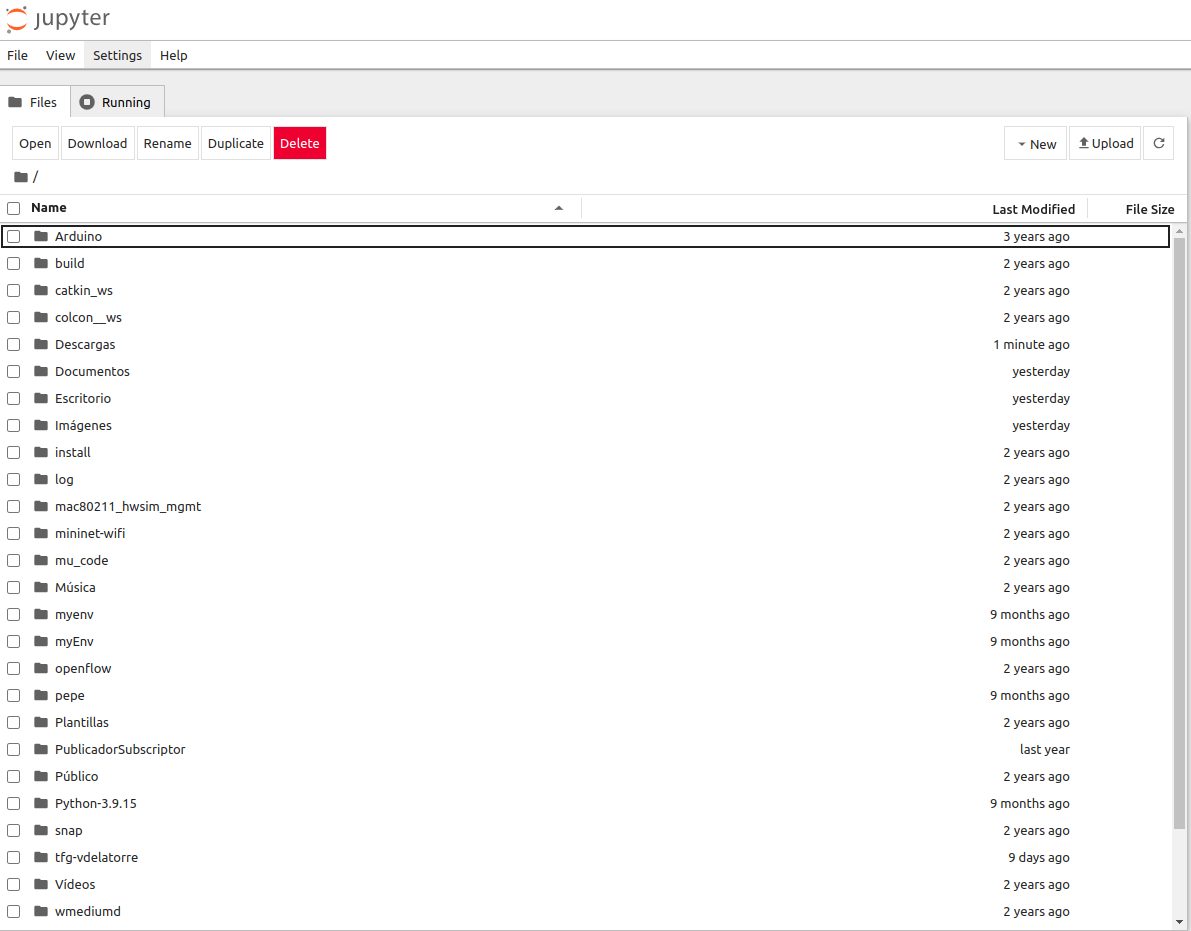
\includegraphics[scale=0.4]{figs/jup1} % Escala la imagen al 150% de su tamaño original
  \caption{Interfaz Jupyter Notebook.}
  \label{fig:jup1}
\end{figure}

Esta herramienta también sirve para manejar bases de datos de prueba y entrenamiento con modelos de aprendizaje automático, ya que se pueden cargar datos y procesarlos de manera interactiva, lo cual será muy útil para hacer las correspondientes pruebas sobre cuántos APs son necesarios para que el robot pueda localizarse como se verá más adelante, ya que para esto se necesitará recoger una gran cantidad de datos de cada APs para que cada modelo procese todo y entorno será de gran ayuda.




\begin{figure}[H]
  \centering
  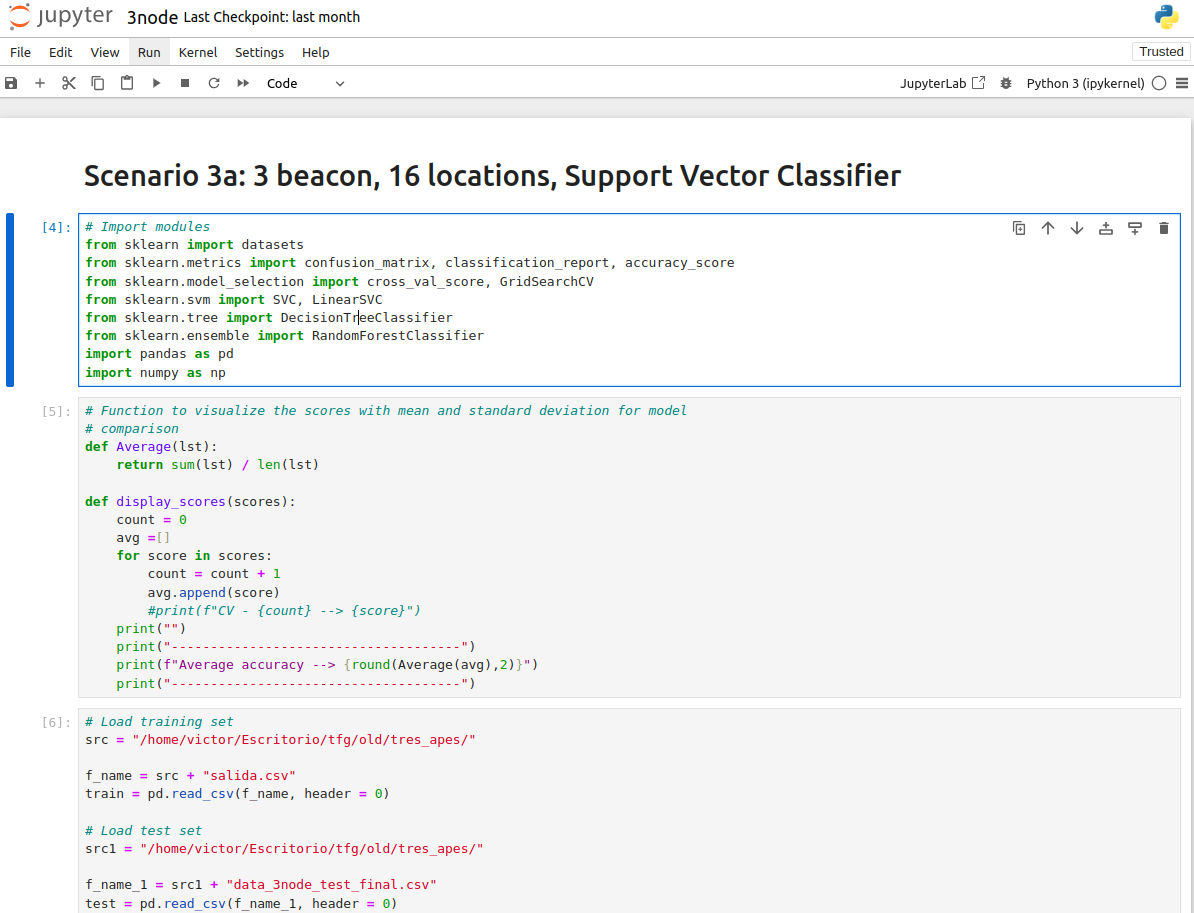
\includegraphics[scale=0.4]{figs/jup2} % Escala la imagen al 150% de su tamaño original
  \caption{Ejemplo de un programa en Jupyter Notebook.}
  \label{fig:jup2}
\end{figure}

\subsection{GIMP}
\label{subsec:gimp}

GIMP es un programa de edición de imágenes de software libre y gratuito en el cual se pueden editar imágenes digitales en forma de mapa de bits, tanto fotografías como dibujos. Para este proyecto, se usará para diseñar el mapa del robot, es decir, dibujar en una imagen píxel a píxel los obstáculos por donde no podrá desplazarse el robot. Para ello se puede hacer uso de las diferentes herramientas como el pincel, lápiz o el borrador y después una vez dibujado el mapa se podrá exportar como una imagen en un formato determinado y ejecutar un programa que hace uso de la Clase Image del módulo PIL que es una biblioteca para trabajar con imágenes en Python y de esta manera poder abrir la imagen, obtener sus dimensiones e iterar sobre cada píxel para escribir la representación binaria, guardarla en formato txt y así esta matriz será la que se le pasará al algoritmo A* para encontrar el camino más óptimo.


\paragraph{Bibliotecas auxiliares utilizadas} \hspace{0pt} \\

A parte de los módulos y bibliotecas mencionadas anteriormente, también se usaron otras herramientas de propósito general. La biblioteca \texttt{threading} la cual se usó para implementar programación concurrente y poder manejar diferentes programas a la vez, como la obtención del ángulo de orientación, mientras que \texttt{subprocess} sirvió para ejecutar comandos externos desde Python, como ejecutar el comando para conectarse a una red WiFi o para grabar un archivo de audio. Para el análisis y manipulación de los datos de audio, se usaron \texttt{pandas} y \texttt{numpy}, que son ampliamente usadas en el ámbito científico. La biblioteca \texttt{heapq} facilitó la gestión eficiente de las estructuras de datos basadas en montículos(heaps), que en este caso se usó sobre todo para manejar el algoritmo A* de una manera más óptima y \texttt{deque} se usó para obtener las útimas lecturas del magnetómetro. Finalmente, se utilizó \texttt{matplotlib.pyplot} para generar y guardar imágenes que ilustraban los resultados obtenidos del algoritmo.\\

Se recomienda instalar todos los paquetes necesarios en un entorno virtual que es un directorio con su propia instalación de Python y sus paquetes, ofreciendo así un control preciso sobre las dependencias de software, el aislamiento de entornos de trabajo y la capacidad de experimentar y probar configuraciones sin afectar al sistema operativo principal, por lo que sería útil instalar la biblioteca \texttt{virtualenv}.


